\chapter{Mezuro}

\section{Métricas de Código-Fonte}

% TODO: Falar um pouco mais sobre métricas

Métricas de código estão ligadas ao desenvolvimento, planejamento, custos,
produtividade e qualidade do software. Existem dois grandes conjuntos delas:
métricas tradicionais e métricas de orientação a objetos. São métricas
tradicionais: métricas de tamanho (ex. Linhas de Código - LOC), métricas de
complexidade (ex. Complexidade Ciclomática), métricas manutenibilidade, dentre
outras (Tamanho Médio dos Módulos, Uso de Variável, Número de Funções, por
exemplo). E são métricas de orientação a objetos: métricas de classes (ex.
Encapsulamento dos Atributos), métricas de métodos (ex. Média de Complexidade
dos Métodos), métricas de acoplamento (ex. Acoplamento Aferente), métricas de
herança (ex. Medida de Polimorfismo) e métricas de sistema (ex. Reúso de
Classe) \cite{meirelles2013monitoramento}.

\section{O Mezuro}

O Mezuro foi planejado para ser uma ferramenta de extração, análise e
interpretação de métricas de código-fonte. De uma forma geral, ele é dividido
em duas partes: para o processamento e para o cálculo é utilizado o Kalibro, que
é um \textit{webservice}; e o Prezento para a interface gráfica (uma aplicação
\textit{Web}) \cite{meirellesCibse2015}. Sob a licença
\textit{Affero General Public License version 3} (AGPLv3), o Mezuro permite que
o usuário crie, salve e edite ``configurações'' que são um conjunto de
métricas escolhidas por este e um ``grupo de leitura'' para provimento de uma
interface gráfica de um conjunto de leitura que tenha algum sentido quando
agrupadas, por exemplo: com a pontuação x, a métrica terá o ``rótulo'' ``BOM'' e
será atribuído a ela a cor amarela; com a pontuação x + 2, a métrica terá o
``rótulo'' ``ÓTIMO'' e estará com a cor verde. As cores são para destacar a
interpretação e são definidas com valores hexadecimal \cite{camarinhaOSS2015}.

O Kalibro, citado no parágrafo anterior, foi inicialmente escrito em Java para
compor uma das ferramentas do projeto QualiPSo (\textit{Quality Platform for
Open Source Software}). Já possuía a maioria das funcionalidades presentes na
versão atual do Mezuro. Uma delas, bastante prática, é a de fornecer apenas o
URL do código compactado em arquivo ZIP ou TARBALL, ou o link para as
aplicações de controle de versão em SVN ou GIT, mais a escolha de uma
configuração, para iniciar a análise \cite{camarinhaOSS2015}. Em 2013 o Mezuro
passou a ser reescrito em Ruby, com objetivo de manter na mesma tecnologia as
camadas da arquitetura. Mudança justificada também pela necessidade do
processamento dos cálculos e da análise. A carga de requisições, mais a
quantidade de núcleos que o servidor possuía, faziam com que a versão original
do Kalibro ficasse debilitado em seu fluxo de execuções. Outra vantagem dessa
reescrita é a facilidade com que novos contribuidores puderam/poderão entender
todo o funcionamento dessa parte do Mezuro. Algumas funcionalidades foram
eliminadas por serem consideradas não essenciais. E grande parte da primeira
versão do Kalibro está presente na gema
kalibro\_gem\footnote{\url{https://rubygems.org/gems/kalibro_gem}}
\cite{meirellesCibse2015}.

% TODO: a gem kalibro\_gem e a kalibro\_client são a mesma coisa? A kalibro\_gem
% foi descontinuada?)

% Sobre o Prezento

O Kalibro foi construído, nos primórdios, como um plugin da rede social
Noosfero. Com a decisão de reescrevê-lo em Ruby, a antiga interface gráfica,
que era aproveitada do Noosfero, foi também reescrita nesta
tecnologia. O Prezento, desenvolvido utilizando o \textit{framework} para
desenvolvimento de aplicações \textit{Web}
Ruby on Rails\footnote{\url{http://guides.rubyonrails.org/getting_started.html}},
é a redesenhada e atual interface.

% Sobre a arquitetura do Mezuro

% (Eu preciso falar do QualiPSo?  Não!)

O projeto QualiPSo, iniciado em meados de 2007, tinha como objetivo aprimorar
as práticas de desenvolvimento aberto à época para atingir o reconhecimento e
confiabilidade que o FOSS possui hoje \cite{messias2012}.

\subsection{Arquitetura e principais funcionalidades do Mezuro}

Com a reescrita, a arquitetura do Mezuro foi dividida em três serviços:

\begin{itemize}
  \item \textit{Prezento}: para a interface gráfica do usuário
  \item \textit{Kalibro Processor}: para a análise do código
  \item \textit{Kalibro Configurations}: para o gerenciamento das configurações
\end{itemize}

A decisão de dividir o Kalibro em serviços separados foi tomada para deixar
cada um deles com menos responsabilidades, facilitando a manutenção e evolução
\cite{camarinhaOSS2015}. E a comunicação entre estes serviços é feita através
do Kalibro Client: um quarto software também escrito em Ruby, mantendo a
escolha de centralização em uma única tecnologia. E para simplificar a
implementação, também foi decidido que a comunicação entre os serviços seria
RESTful.

As figuras a seguir demonstram como a comunicação funciona, um diagrama UML de
sequência do processo de criação de uma configuração chegando ao estágio em que
são expostos os resultados finais de uma análise após a reescrita da interface
gráfica, e outra que demonstra o estado atual do projeto.

\begin{figure}[!htb]
	\centering
    \includegraphics[keepaspectratio=true,scale=0.5]
    {figuras/mezuroCloudArch.eps}
  \caption{Arquitetura do Mezuro \cite{camarinhaOSS2015}}
	\label{fig:mezuroNoosferoArch}
\end{figure}

\begin{figure}[!htb]
	\centering
    \includegraphics[keepaspectratio=true,scale=0.7]
    {figuras/prevProcessingSeqDiag.eps}
  \caption{Arquitetura do sistema ao fim da reescrita da interface gráfica
  \cite{meirellesCibse2015}}
	\label{fig:prevProcessingSeqDiag}
\end{figure}

\begin{figure}[!htb]
	\centering
    \includegraphics[keepaspectratio=true,scale=0.5]
    {figuras/processingSeqDiag.eps}
  \caption{Arquitetura do sistema ao fim da reestruturação do Kalibro
  \cite{meirellesCibse2015}}
	\label{fig:processingSeqDiag}
\end{figure}

\newpage

Segundo \citeonline{camarinhaOSS2015}, as principais ``funcionalidades podem ser
divididas em dois grupos:

\begin{itemize}
  \item Projeto
    \begin{itemize}
    \item \textit{Download} do código-fonte a partir de repositórios (Git,
    Subversion, Bazaar etc) ou via arquivo compactado;
        \item Escolha da periodicidade do processamento do código (1 dia, 2 dias,
        semanal, quinzenal e mensal);
        \item Escolha de qual configuração de métricas cada repositório irá
        utilizar;
        \item Nota de cada métrica da configuração para cada arquivo do
        repositório;
        \item Análise gráfica de cada arquivo do repositório por meio de um
        gráfico de pontos com notas ao longo do tempo;
        \item Resultados públicos e acessíveis à comunidade.
    \end{itemize}
    \item Configuração
    \begin{itemize}
    \item Criação de configuração e a possibilidade de clonagem;
        \item Estatísticas sobre as configurações mais populares dentro da
        comunidade;
        \item Criação de intervalos qualitativos associados aos valores das
        métricas;
        \item Criação de grupos de leitura para a interpretação textual dos
        resultados das métricas;
        \item Combinações de métricas nativas para criação de análises compostas
        e mais complexas.''
    \end{itemize}
\end{itemize}
''
% TODO: consertar estas aspas na citação direta

\newpage

\section{Mezuro: Prezento}

O Prezento é a camada da interface web do
Mezuro. Desenvolvido em Ruby on Rails, atualmente utiliza as versões 2.3.0 do
Ruby e 4.2.4 do Rails. Versões estas que estão em constante mudança, pois os
autores têm como intuito usufruir o que há de mais recente das funcionalidades
dessa tecnologia. Esta será a principal camada trabalhada neste trabalho de
conclusão de curso, pois é
nela que há a interação com o usuário. Possivelmente será utilizado um botão que
possibilitará ao usuário ter acesso e interação com a visualização gráfica do
resultado da análise estática na mesma página ou em outra. As Figuras
\ref{fig:exmplo_disposicao_botao_visualizacao_1} e
\ref{fig:exmplo_disposicao_botao_visualizacao_2} mostram possíveis localizações
para este botão.

% TODO: atualizar estas imagens e DESTACAR botões

\begin{figure}[!htb]
	\centering
    \includegraphics[keepaspectratio=true,scale=0.33]
    {figuras/exmplo_disposicao_botao_visualizacao_1.eps}
  \caption{Possíveis disposições dos botões de acesso à visualização (recolhido)}
  \label{fig:exmplo_disposicao_botao_visualizacao_1}
\end{figure}

\begin{figure}[!htb]
	\centering
    \includegraphics[keepaspectratio=true,scale=0.33]
    {figuras/exmplo_disposicao_botao_visualizacao_2.eps}
  \caption{Possíveis disposições dos botões de acesso à visualização
  (expandido) (adptado) \cite{filgueiras2014mezuro}}
  \label{fig:exmplo_disposicao_botao_visualizacao_2}
\end{figure}

\newpage

As Figuras \ref{fig:controllers_complete} e \ref{fig:models_complete} mostram os
diagramas das camadas de Controle e de Modelo do Prezento. Foram geradas com a
\textit{gem} RailRoady\footnote{\url{http://railroady.prestonlee.com/}}.

% TODO: atualizar estes diagramas

\begin{figure}[!htb]
	\centering
    \includegraphics[keepaspectratio=true,scale=0.33]
    {figuras/controllers_complete.eps}
  \caption{Diagrama da Camada de Controle}
  \label{fig:controllers_complete}
\end{figure}

\begin{figure}[!htb]
	\centering
    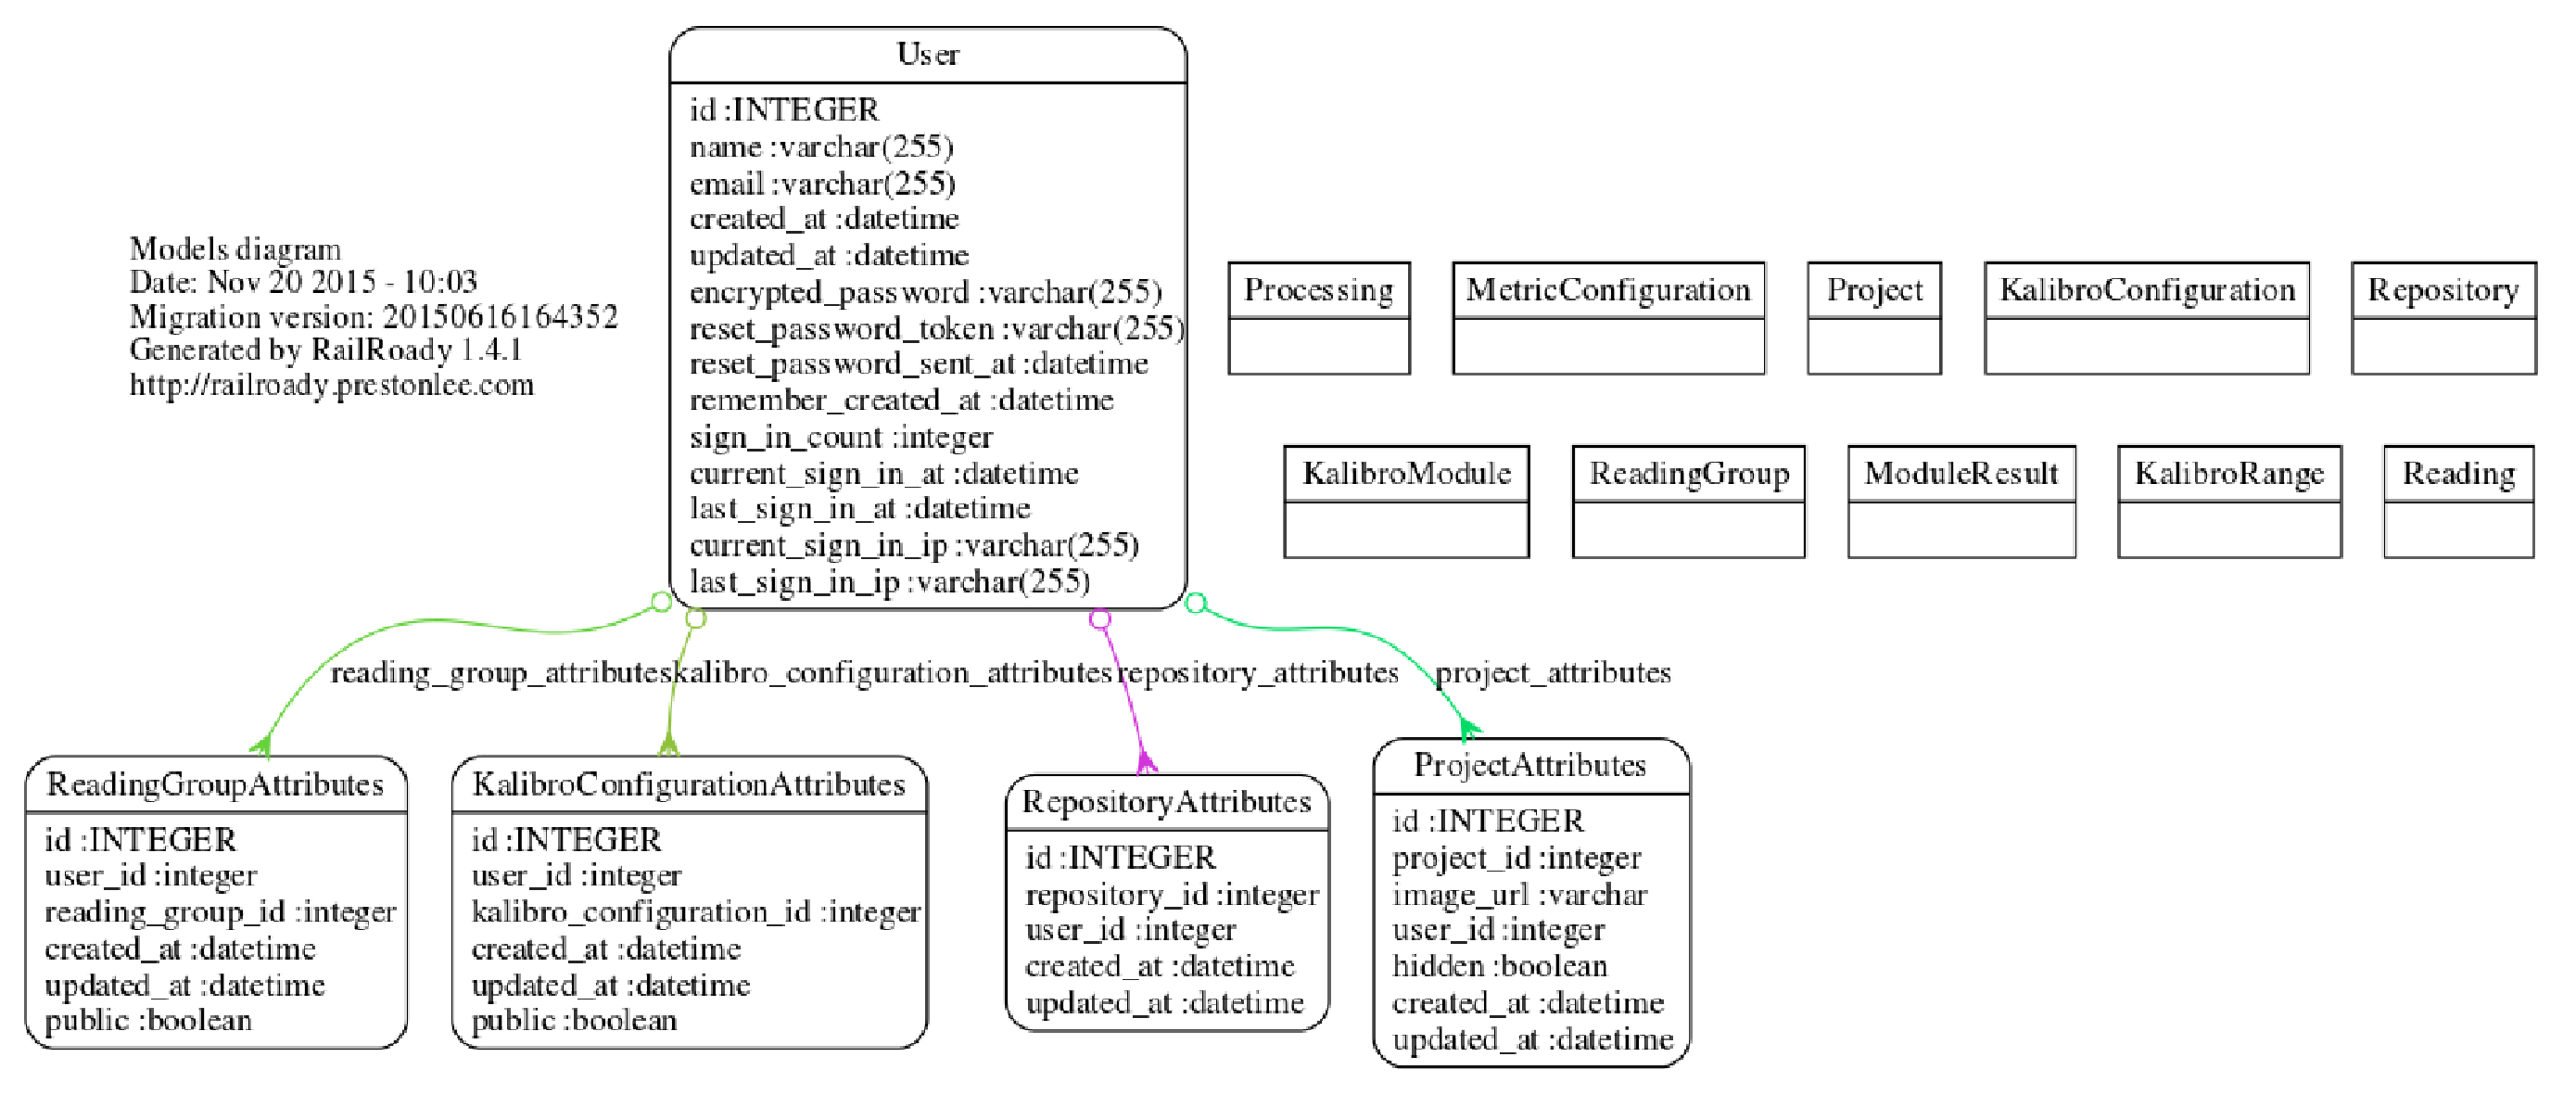
\includegraphics[keepaspectratio=true,scale=0.35]
    {figuras/models_complete_v2.eps}
  \caption{Diagrama da Camada de Modelo}
  \label{fig:models_complete}
\end{figure}

\section{A Decisão de utilizar o Mezuro}

Para este trabalho de conclusão de curso a ferramenta de análise de código
fonte escolhida foi o Mezuro pois: o aluno já participou da evolução de parte
de algumas funcionalidades; a ferramenta proporciona ao usuário a análise
periódica do projeto, o que atende ao desejado como contribuição tecnológica
das visualizações geradas serem demonstradas ao longo do tempo; por ser uma
plataforma livre; fácil contato com os mantenedores; e por esta plataforma
sempre utilizar as últimas versões estáveis do Ruby e do Rails, ou seja,
por utilizar o que há de mais atual nestas tecnologias.

É importante ressaltar que outras ferramentas de análise de código poderão ser
utilizadas para geração da visualização proposta neste trabalho. Pois o fluxo
básico de execução permitirá tal geração, a saber: análise pela ferramenta,
dados exportados de forma determinada para atender a leitura da biblioteca JS,
geração da visualização em um terceiro serviço local ou remoto.

E o ideal é que este trabalho sirva como base para a criação de futuras
visualizações para o Mezuro em si.

O foco do desenvolvimento, por tanto, será na camada de \textit{GUI} do Mezuro,
chamada Prezento.
